
\subsection{Perfektní grafy}

\df (Perfektní graf) Graf je perfektní, pokud pro každý jeho indukovaný podgraf 
platí, že $\chi(G) = \omega(G)$. Některé třídy perfektních grafů jsou:
\begin{itemize}
	\item Bipartitní grafy (pokud obsahují hranu, jsou vždy dvoubarevné).
	\item Chordální grafy (obarvit podle perfektního eliminačního schématu, 
		které nachází maximální kliku).
\end{itemize}

\vt (Lovász) Graf je perfektní právě tehdy, když je jeho doplněk perfektní.

\vt (Berge) Graf je perfektní právě tehdy, když neobsahuje díry (liché cykly) 
ani antidíry (doplňky lichých cyklů) jako indukovaný podgraf.  (Lichý cyklus ani 
doplněk nemůže být perfektní, protože potřebuje 3 barvy, ale má kliku velikosti 
max. 3, opačná implikace je těžká)

\subsection{Barevnost a maximální stupeň}

\vt (Brooksova věta.) Pro souvislý neorientovaný graf $G$ s maximálním stupněm 
$\Delta$ platí, že $\chi(G) \leq \Delta$, pokud nejde o úplný graf nebo lichý 
cyklus (v takovém případě je triviálně $\chi(G) = \Delta+1$.
\dk Indukcí podle velikosti. Pro $n = \Delta$ platí triviálně.  Předpokládáme 
regulární graf (jinak odebereme vrchol menšího stupně, použijeme indukci a 
vrchol dobarvíme). Pokud je $i$ nebo $2$-souvislý, obarvíme komponenty zvlášť 
indukcí. U 3-souvislého grafu nejdeme vrchol s maximálním stupněm $u$, jeho dva 
sousedy $v,w$ nespojené hranou (existují pokud není úplný), vytvoříme kostru 
$G-\{v,w\}$ zakořeněnou v $u$, vrcholy $v,w$ dodáme nakonec a obarvíme hladově 
od listů.  Protože každý vrchol až na $u$ má otce v kostře, zbyde na něj
barva. Na $u$ zbyde proto, že $v$ a $w$ mají stejnou barvu.

\vt (Vizingova) Pro libovolný graf $G$ bez smyček a násobných hran platí: 
$\Delta(G) \leq \chi'(G) \leq \Delta(G) +1$, kde $\chi'$ je hranová barevnost.
{\it Důkaz je indukcí podle počtu hran. Pro hranu $e$ se obarví graf $G-e$ a 
	hrana $e$ se dobarví na volnou barvu z obou vrcholů. Pokud taková není, 
hledá se kde prohodit barvy na střídavé cestě.}

\subsection{Barevnost a girth}

\vt (Grötszchova věta.) Každý rovinný graf bez trojúhelníků je 3-obarvitelný.  
{\it Discharging argument: uvažuje se minimální protipříklad, který neobsahuje 
	zakázané (nereducibilní) konfigurace. Přiřazením záporného náboje a 
distribucí za předpokladu, že konfigurace nejsou obsaženy se získá kladný náboj, 
a to je spor.}.

% MAT307
\vt (O vztahu barevnosti a girth.) Pro každé $k$ a $l$ existuje graf s 
chromatickým číslem $> k$ a girth $>l$. Speciálně omezením girth nezískáme málo 
barevné grafy.

\dk {\it (pouze pro grafy bez trojúhelníků)} Začneme s hranou, to jest $G_2$ 
(potřebuje 2 barvy).  Vybudujeme $G_{n+1}$ tak, že přidáme nový vrchol $z$, 
zdvojíme všechny vrcholy, kopie spojíme hranou se sousedy svých předloh a $z$.  
Takový graf je bez trojúhelníků, které mohly vzniknout jenom se $z$ a žádní 
sousedi $z$ nemají mezi sebou hranu (konstrukce na obrázku 
\ref{triangle-free-colorful-construction}).  Protože obě části vrcholů lze 
obarvit stejně, triviálně umíme obarvit graf $n+1$ barvami.  Předpokládejme, že 
$G_n$ potřeboval $n$ barev.  Potom pro každou barvu $c$ existuje vrchol, který 
ji má vynucenou v $G_n$; jeho klon ji ale má vynucenou v $G_{n+1}$ také, protože 
sdílí sousedy -- nelze ji tedy využít pro obarvení $z$.
\begin{figure}[h!]
	\centering
	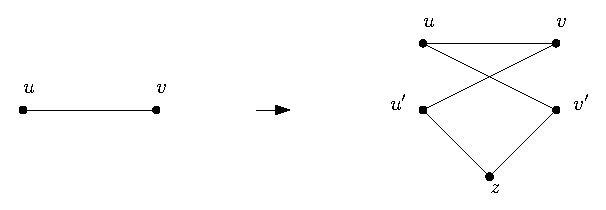
\includegraphics{img/triangle-free-colorful-construction.eps}
	\caption{Postup od $G_2$ na $G_3$}
	\label{triangle-free-colorful-construction}
\end{figure}

\subsection{Vybíravost}

\df (Barvení ze seznamů) Graf je obarvitelný ze seznamů $S_v$ povolených barev 
pro každý vrchol, pokud lze vybrat pro každý vrchol barvu z jeho seznamu 
takovou, že sousední vrcholy mají různou barvu.

\df (Vybíravost) Graf je $k$-obarvitelný, pokud ho lze obarvit ze seznamů délky 
$k$. Graf je $k$-vybíravý, pokud $k$ je nejmenší takové, aby byl 
$k$-obarvitelný.

\vt (Thomassen) Každý rovinný graf je 5-vybíravý.

\dk Zavedeme indukční předpoklad: 

{\it Pro rovinný graf $G$, který se skládá z vnějšího cyklu $C$, na kterém jsou 
	dva sousední vrcholy předbarvené, a vnitřní stěny jsou triangulace, lze 
	rozšířit toto předbarvení na celý graf pokud všechny vrcholy na $C$ mají 
seznam délky alespoň $3$ a všechny vnitřní vrcholy alespoň $5$.}

Graf tedy doplníme na triangulaci, určíme vnější stěnu a hodíme graf do indukce 
podle počtu vrcholů. Pokud má graf chordu, rozdělíme ho podle ní na dvě 
poloviny, aplikujeme indukci na každou zvlášť, nejdříve však na půlku, která má 
předbarvené vrcholy. Pokud chordu nemá: předpokládáme $C=\{v_1, \dots, v_k\}$ 
vrcholy na vnější stěně, $v_1$ a $v_2$ jsou již obarvené, obarvíme $v_k$: 
zvolíme dvě barvy ze seznamu $v_k$, vyškrtáme
je z jeho sousedů uvnitř grafu $u_i$ (ti měli 5, zbydou jim alespoň 3, tak 
akorát do indukce) a graf pustíme dál do indukce bez $v_k$ (viz obrázek).  
Následně obarvíme $v_k$ barvou, kterou nepoužil $v_{k-1}$, takové máme dvě, 
které jsme si vyškrtali ze sousedů $u_i$ kromě $v_{k-1}$!

\noindent
\begin{figure}[h!]
	\centering
	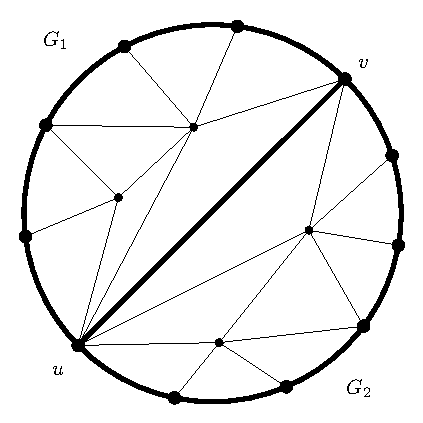
\includegraphics{img/thomassen-chord.eps}
	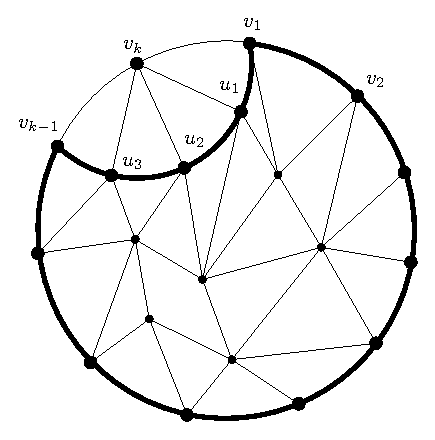
\includegraphics{img/thomassen-induction.eps}
	\caption{Postup indukce v grafu s chordou a bez ní.}
\end{figure}

\vt (List Coloring Conjecture) Pro každý graf platí $\chi'(G) = ch'(G)$.

\vt (Galvin) Pro každý bipartitní graf platí $\chi'(G) = ch'(G)$.

\subsection{Kernel}

\df (Kernel) Nezávislá množina $U$ v orientovaném grafu je {\it kernel}, pokud 
každý vrchol $v\in G \setminus U$ má hranu $vu$ do nějakého vrcholu $u\in U$.  
{\it Alternativně: každý vrchol je v kernelu, nebo do něj má hranu.}

\lm Nechť $G$ je graf a $D$ jeho orientace a každý vrchol má méně výstupních 
hran, než barev ve svém seznamu, a každý indukovaný podgraf $D$ má kernel, potom
má $G$ seznamové obarvení.

\dk Pro barvu $\alpha$ vezmu graf indukovaný vrcholy, které mají $\alpha$ ve 
svých seznamech. Z předpokladů tento graf má kernel -- obarvím kernel barvou 
$\alpha$, odstraním a pokračuji indukcí (graf se zmenšil, některým vrcholům se 
zmenšily seznamy, ale také ekvivalentně odchozí stupně -- předpoklady stále 
platí).
